%% LyX 2.2.3 created this file.  For more info, see http://www.lyx.org/.
%% Do not edit unless you really know what you are doing.
\documentclass[english]{article}
\usepackage[T1]{fontenc}
\usepackage[latin9]{inputenc}
\usepackage{geometry}
\geometry{verbose,tmargin=1in,bmargin=1in,lmargin=1in,rmargin=1in,headheight=0in,headsep=0in}
\usepackage{graphicx}
\usepackage{babel}
\usepackage[unicode=true]
 {hyperref}

\makeatletter

%%%%%%%%%%%%%%%%%%%%%%%%%%%%%% LyX specific LaTeX commands.
%% Because html converters don't know tabularnewline
\providecommand{\tabularnewline}{\\}

\makeatother

\begin{document}
\begin{center}
\textbf{\Large{}CSCE 221 Cover Page}{\Large{}}\\
{\Large{} Homework Assignment \#3}\\
{\Large{}Due April 25 at 23:59 pm to eCampus}\bigskip{}
\par\end{center}

First Name~~~~~Hunter~~~~~~Last
Name ~~~Cleary~~~~UIN~~~625001547~~~\bigskip{}

User Name ~~~hncleary~~~~E-mail
address~~~~hncleary@tamu.edu~~~~~~~\medskip{}

Please list all sources in the table below including web pages which
you used to solve or implement the current homework. If you fail to
cite sources you can get a lower number of points or even zero, read
more on Aggie Honor System Office website: \texttt{\href{http://aggiehonor.tamu.edu/}{http://aggiehonor.tamu.edu/}}\medskip{}
\medskip{}
\noindent \begin{flushleft}
\begin{tabular}{|c|c|c|c|c|}
\hline 
Type of sources  & ~~~~~~~~~~~~~~~~~~~~~~~ & ~~~~~~~~~~~~~~~~~~~~~~~~ & ~~~~~~~~~~~~~~~~~~~~~~~ & ~~~~~~~~~~~~~~~~~~~~~~~\tabularnewline
 &  &  &  & \tabularnewline
\hline 
People &  &  &  & \tabularnewline
 &  &  &  & \tabularnewline
\hline 
Web pages (provide URL)  & Listed Below  &  &  & \tabularnewline
 &  &  &  & \tabularnewline
\hline 
Printed material & Data Structures and Algorithms &  &  & \tabularnewline
 & (Textbook) &  &  & \tabularnewline
\hline 
Other Sources  &  &  &  & \tabularnewline
 &  &  &  & \tabularnewline
\hline 
\end{tabular}
\par\end{flushleft}
https://en.wikipedia.org/wiki/Eulerian\_path\ \\
https://en.wikipedia.org/wiki/Dijkstra\%27s\_algorithm\ \\
https://www.geeksforgeeks.org/greedy-algorithms-set-6-dijkstras-shortest-path-algorithm/\ \\
https://en.wikipedia.org/wiki/Double\_hashing\ \\

\medskip{}
\medskip{}

\noindent I certify that I have listed all the sources that I used
to develop the solutions/codes to the submitted work.

\noindent \emph{On my honor as an Aggie, I have neither given nor
received any unauthorized help on this academic work}.

\bigskip{}
\bigskip{}

\begin{tabular}{cccccc}
Your Name  & ~~~Hunter~Cleary~~~~ &  & ~~~~~~~~~~~~~~~~~~~~~ & Date  & ~~~4/24/18~~~~\tabularnewline
\end{tabular}

\begin{center}
\newpage{}\textbf{Homework 3 (100 points)}
\par\end{center}

\begin{center}
\textbf{due April 25 at 11:59 pm to eCampus.}
\par\end{center}

\begin{flushleft}
Write clearly and give full explanations to solutions for all the
problems. Show all steps of your work. 
\par\end{flushleft}

\begin{flushleft}
\textbf{Reading assignment.}
\par\end{flushleft}
\begin{itemize}
\item Hash Tables Chap. 9
\item Heap and Priority Queue, Chap. 8
\item Graphs, Chap. 13
\end{itemize}
\textbf{Problems.}
\begin{enumerate}
\item (10 points) R-9.7 p. 417

Draw the 11-entry hash table that results from using the has function,
$h(k)=(3k+5)$ mod 11, to hash the keys 12, 44, 13, 88, 23, 94, 11,
39, 20, 16, and 5, assuming collisions are handled by chaining.\ \\
\ \\
$h(k) = (3k+5)\%11$\ \\
$h(12) = 8 , \ h(44) = 5, \ h(13) = 0, \ h(88) = 5, \ h(23) = 8, \ h(94) = 1, \ h(11) = 5, \ h(39) = 1, \ h(20) = 10, \ h(16) = 9, \ h(5) = 9$
\ \\
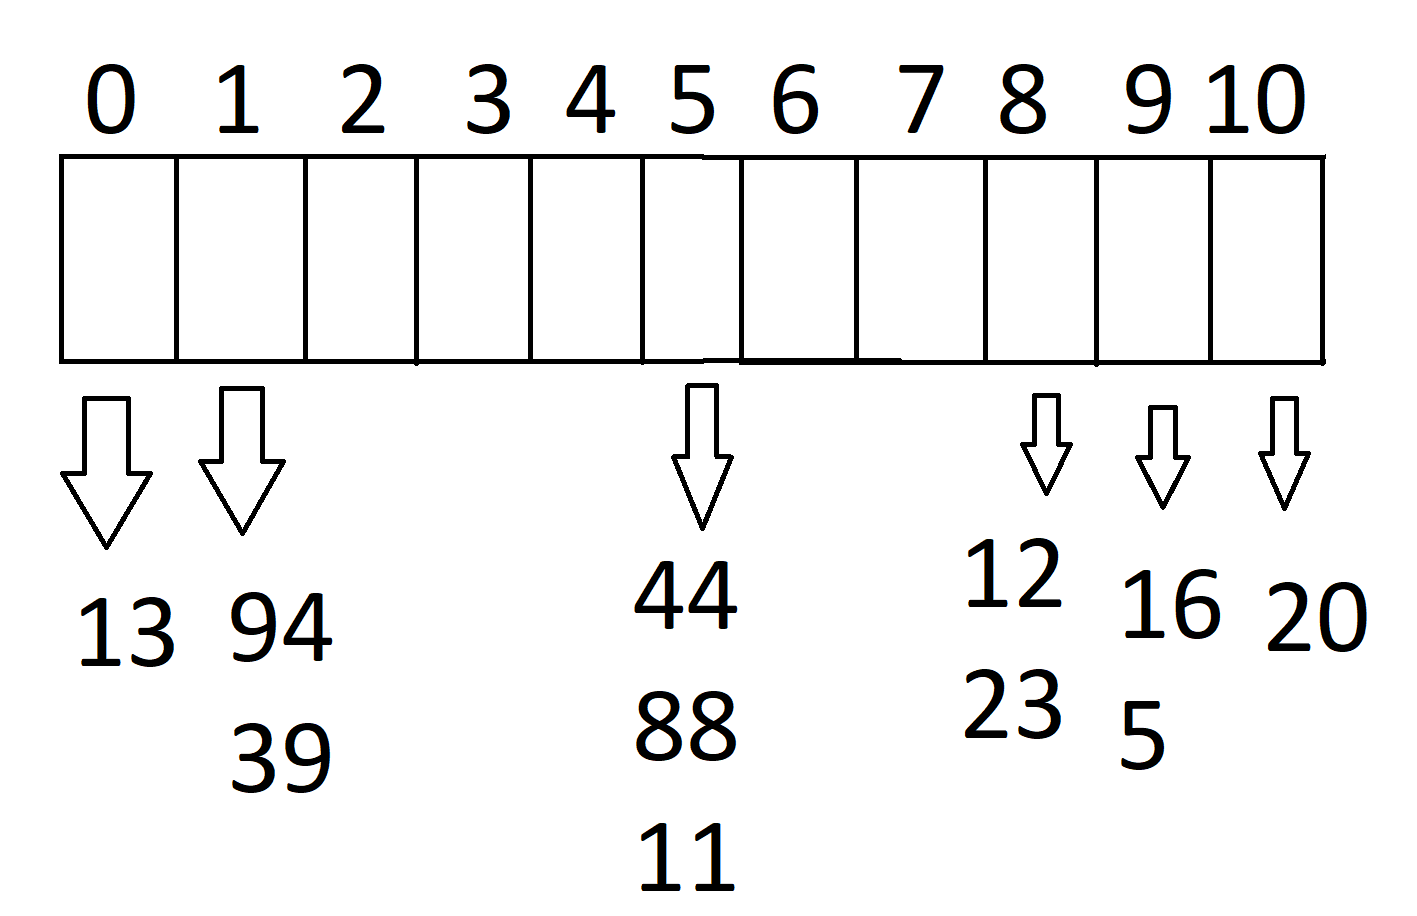
\includegraphics[width=12cm,height=\textheight,keepaspectratio]{Homework3HashTable.png}\ \\
\ \\
\item (10 points) R-9.8 p. 417
What is the result of the previous exercise, assuming collisions are
handled by linear probing?\ \\
\ \\
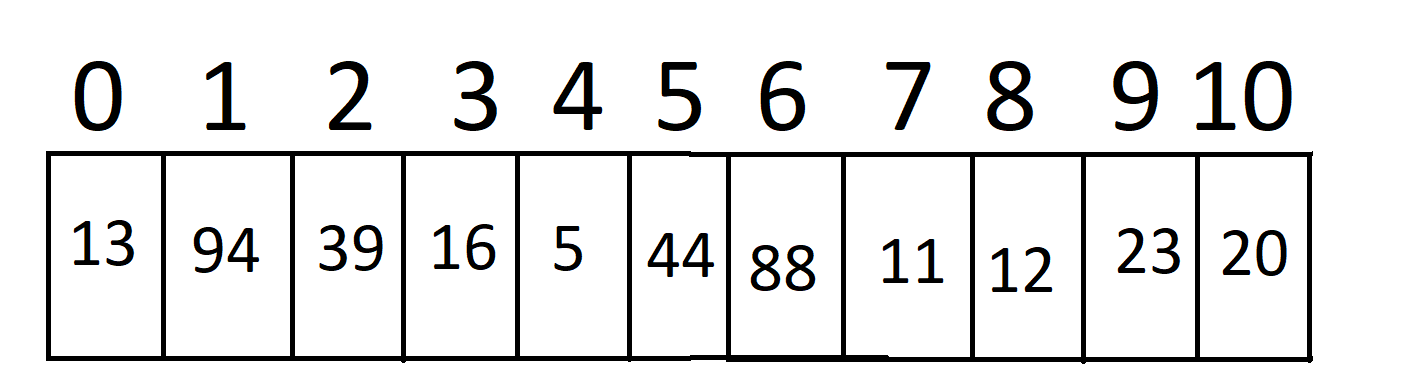
\includegraphics[width=12cm,height=\textheight,keepaspectratio]{Homework3HashTableProbing.png}\ \\
\ \\
\item (10 points) R-9.10 p. 417 

What is the result of Exercise R-9.7, when collisions are handled
by double hashing using the secondary hash function $h_{s}(k)=7-(k$
mod $7)$?\ \\
\ \\
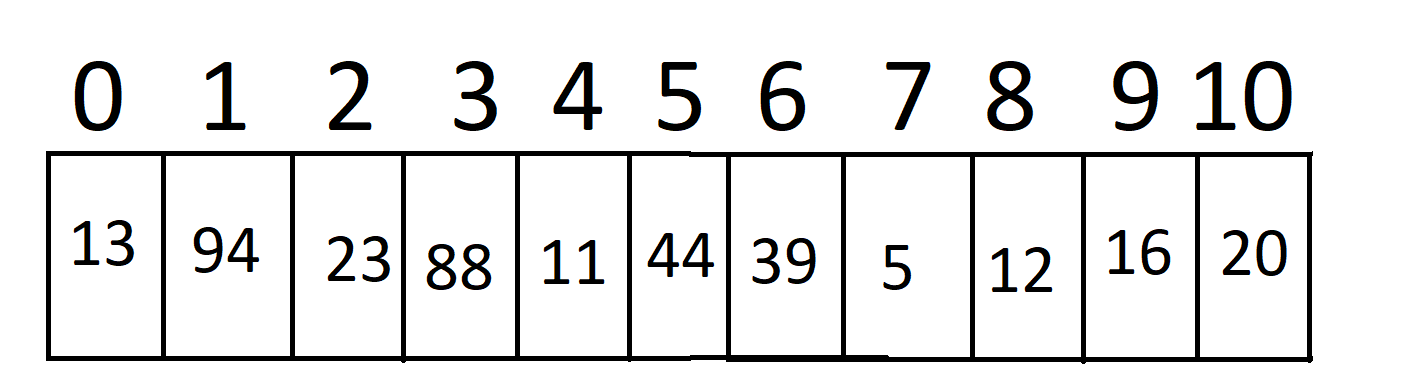
\includegraphics[width=12cm,height=\textheight,keepaspectratio]{Homework3HashTableDoubleHashing.png}\ \\

\ \\
\item (10 points) R-8.7 p. 361\ \\
An airport is developing a computer simulation of air-traffic control
that handles events such as landings and takeoffs. Each event has
a \emph{time-stamp }that denotes the time when the event occurs. The
simulation program needs to efficiently perform the following two
fundamental operations:
\begin{itemize}
\item Insert an event with a given time-stamp (that is, add a future event)
\item Extract the event with smallest time-stamp (that is, determine the
next event to process)
\end{itemize}
Which data structure should be used for the above operations? Why?
Provide big-oh asymptotic notation for each operation.\ \\
\ \\
\textbf{Solution}\ \\
The data structure that should be used for this scenario is a binary heap. The heap is made up of nodes that have a key and an element. These will correspond to the time and the event.\ \\
\ \\
Insertion and search for the binary heap wold both be done in $O(logn)$ time.
%\newpage\ \\
\ \\
\item (10 points) R-13.5, p. 654\ \\
\ \\
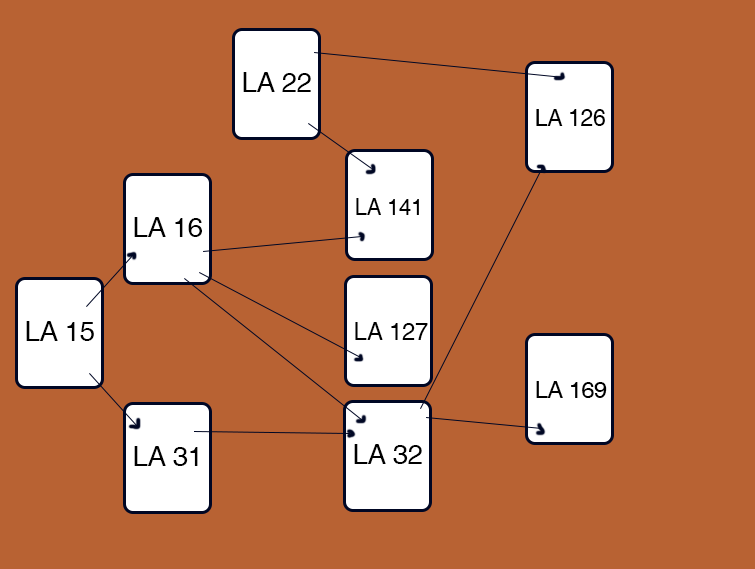
\includegraphics[width=8cm,height=\textheight,keepaspectratio]{Problem5Chart.png}\ \\
\ \\
$LA15 -> LA16 -> LA31 -> LA22 -> LA141 -> LA127 -> LA32 -> LA169 -> LA126$
\ \\
\ \\
\item (10 points) R-13.7, p. 655\ \\
\ \\
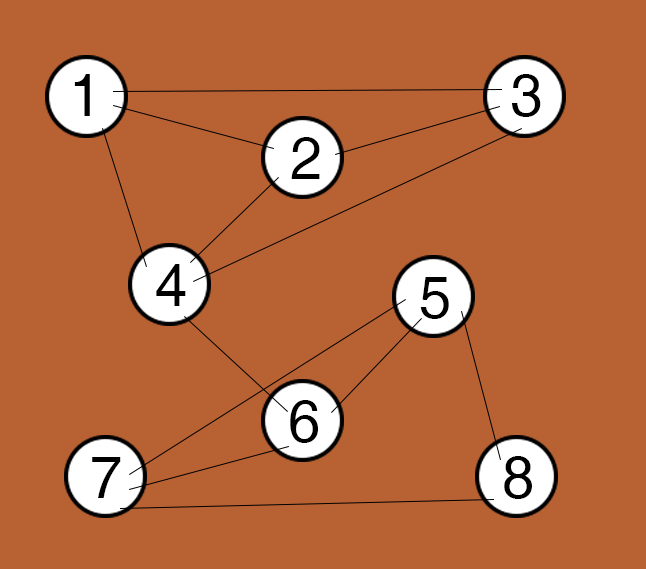
\includegraphics[width=8cm,height=\textheight,keepaspectratio]{Problem6.png}\ \\
\ \\
\textbf{DFS Traversal:} 1 -> 2 -> 3 -> 4 -> 6 -> 5 -> 7 -> 8
\ \\
\textbf{BFS Traversal:} 1 -> 2 -> 3 -> 4 -> 6 -> 5 -> 7 -> 8
\ \\
\item (10 points) R-13.16, p. 656
\ \\
Initialize $D[v] = 0$ and $D[u]=\infty$ for every vertex that isn't the root.\ \\
\ \\
Priority queue contains all vertices of the graph G using keys as labels for D.\ \\
\ \\
For each vertex u, there is a closest u. Whenever a vertex u that isn't the root is removed from the priority queue add an edge (closest to u, u) to the tree.\ \\
\ \\
\item (10 points) R-13.31, p. 657\ \\
\ \\
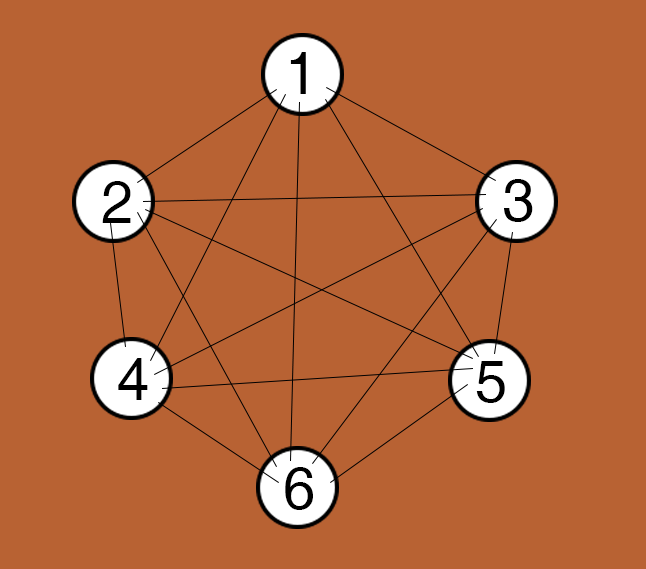
\includegraphics[width=5cm,height=\textheight,keepaspectratio]{Problem8.png}
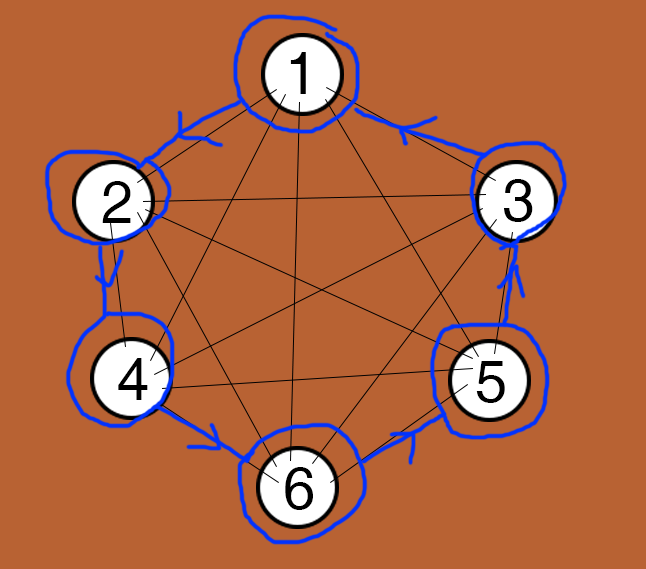
\includegraphics[width=5cm,height=\textheight,keepaspectratio]{Problem8-2.png}\ \\
\ \\
\textbf{DFS Yields:} \ 1 -> 2 -> 4 -> 6 -> 5  -> 3\ \\
\newpage
\item (10 points) C-13.10, p. 658\ \\
\ \\
%for(int i = 1; i <= n ; ++i){
Set a starting vertex v. Find a cycle starting and ending at the starting vertex v so that it contains all edges going into and out of v. Put each edge of the cycle into a list in the order of the cycle. Traverse the list to find the first vertex that has an outgoing edge that is un-visited. If the vertex doesn't have the outgoing edge, then the algorithm is complete. If not, then recursively repeat function with the new edge to create a new cycle.\ \\
\ \\
The algorithm visits and puts into a list each edge in $O(1)$ time. The total time complexity is then $O(m+n)$. m is the number of edges, and n is the number of vertices in the graph.
\ \\
\item (10 points) C-13.15, p. 659\ \\
\ \\
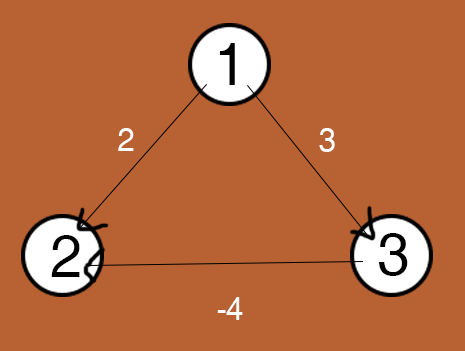
\includegraphics[width=7cm,height=\textheight,keepaspectratio]{Problem10.png}\ \\
\ \\
The algorithm will start on vertex 1. Edges 1 -> 2 and 1 -> 3 will be relaxed first (order is not consequential). These two will be pulled off of the priority queue. Dijkstra's algorithm will determine 2's shortest path to be 1 -> 2, when it is actually 1 -> 3 -> 2.
\ \\
\end{enumerate}

\end{document}
